\chapter{测量、密度矩阵与熵}

双缝实验以最小可用的形式包含了测量问题。当两个备选路径保持相干时，它们的振幅发生干涉。当另一个系统获得了关于实际所取路径的记录时，客体与记录者便发生纠缠，干涉也随之改变。在引入迹、密度矩阵和熵---即量化纠缠所需的语言之前，我们将使这一机制变得精确。

\section{重建双缝实验}

考虑一个离散模型：源位于格点\(0\)，两个开口为\(A\)与\(B\)，屏幕的可能到达位置由正交归一态\(\{|m\rangle\}\)表示。粒子可以是电子、光子或任何其他量子客体。我们称它为电子，并忽略其自旋，使位置成为所讨论的唯一自由度。屏障的其余部分关闭：电子到达除\(A\)或\(B\)以外的任何格点都会被反射。

结构原理是线性性。若两个态按
\begin{equation}
|A\rangle\longrightarrow |A'\rangle,
\qquad
|B\rangle\longrightarrow |B'\rangle,
\end{equation}
演化，则每个叠加态以相同的系数演化：
\begin{equation}
\alpha|A\rangle+\beta|B\rangle
\longrightarrow
\alpha|A'\rangle+\beta|B'\rangle.
\end{equation}

在对称装置中，源以相等振幅向两个开口馈送。如黑板上那样，略去公共归一化因子，
\begin{equation}
|0\rangle\longrightarrow |A\rangle+|B\rangle.
\end{equation}
归一化后的态应为\((|A\rangle+|B\rangle)/\sqrt{2}\)；被略去的因子在干涉论证中不起作用。

现在分别研究每条路径。从开口到屏幕的传播具有如下形式
\begin{align}
|A\rangle &\longrightarrow \sum_m \psi_m|m\rangle, \\
|B\rangle &\longrightarrow \sum_m \phi_m|m\rangle.
\end{align}
复数\(\psi_m\)是从\(A\)出发后到达屏幕格点\(m\)的振幅，而\(\phi_m\)是从\(B\)出发后相应的振幅。

\begin{figure}[htbp]
\centering
\includegraphics[width=0.68\textwidth]{lecture_07_figure_02.png}
\caption{在屏幕基下分别沿\(A\)路径与\(B\)路径的展开。}
\lectureframe{00:05:39}
\end{figure}

若\(B\)关闭，则在\(m\)处的概率为
\begin{equation}
P_A(m)=|\psi_m|^2.
\end{equation}
若\(A\)关闭，
\begin{equation}
P_B(m)=|\phi_m|^2.
\end{equation}
经典概率会建议在两个开口都可用时将这两个结果相加。量子力学则先将振幅相加：
\begin{equation}
|A\rangle+|B\rangle
\longrightarrow
\sum_m(\psi_m+\phi_m)|m\rangle.
\end{equation}
在固定的屏幕格点处，
\begin{align}
P(m)
&=|\psi_m+\phi_m|^2 \\
&=|\psi_m|^2+|\phi_m|^2
  +\psi_m^*\phi_m+\phi_m^*\psi_m.
\end{align}

\begin{figure}[htbp]
\centering
\includegraphics[width=0.70\textwidth]{lecture_07_figure_03.png}
\caption{四项屏幕概率。最后两项是干涉项。}
\lectureframe{00:09:21}
\end{figure}

在对称点处，\(\psi_m=\phi_m\)，两个备选路径相互加强。在相位相差\(\pi\)的点处，\(\psi_m=-\phi_m\)，概率为零。单独任一路径都能到达该点，然而同时打开两条路径却可能阻止电子到达那里。问题现在不可避免：当某物记录了使用了哪个开口时，发生了什么变化？

\section{探测器发生纠缠}

引入一个辅助的二态系统，其态为\(|u\rangle\)与\(|d\rangle\)。在此模型中它不是电子的自旋；它是一个最小的外部装置。初始时探测器未被触发：
\begin{equation}
|0,d\rangle.
\end{equation}
安排相互作用，使得经过\(A\)时探测器翻转，而经过\(B\)时探测器保持不变：
\begin{equation}
|0,d\rangle
\longrightarrow
|A,u\rangle+|B,d\rangle.
\end{equation}
电子离开开口后，不再与辅助自旋相互作用。因此两个分支按如下方式传播
\begin{align}
|A,u\rangle &\longrightarrow \sum_m\psi_m|m,u\rangle, \\
|B,d\rangle &\longrightarrow \sum_m\phi_m|m,d\rangle,
\end{align}
最终态为
\begin{equation}
|\Psi\rangle
=\sum_m\left(\psi_m|m,u\rangle+\phi_m|m,d\rangle\right).
\end{equation}
路径与探测器记录现在处于纠缠之中。读取探测器将揭示使用了哪个开口。

\begin{classroomqa}
\lecturetimestamp{00:13:24}
\audiencequestion{当自旋翻转时，波包是否已经坍缩？}
\lecturerresponse{仅就电子而言，可以使用坍缩语言：路径备选不再干涉。然而对于完整的电子--探测器系统，两个分支都未被丢弃。态仍然是\(|A,u\rangle+|B,d\rangle\)。将装置纳入其中，就把\emph{电子坍缩了}这一说法替换为如下精确陈述：系统--装置之间建立了纠缠。}
\end{classroomqa}

辅助自旋只是一个方便的指针。一个被触发或未被触发的装置、一个被发射或缺失的光子，或任何其他一对可区分的记录，都可以扮演同样的角色。

\begin{classroomqa}
\lecturetimestamp{00:15:17}
\audiencequestion{穿过金属板本身是否总会留下路径记录？}
\lecturerresponse{不一定。关键在于相互作用是否使金属板处于可区分的末态。如果金属板存在激发能隙，而电子没有足够能量激发它，就不必留下持久的内部标记。仅仅发生相互作用是不够的；两个备选路径必须与可区分的记录建立关联。}
\end{classroomqa}

\begin{classroomqa}
\lecturetimestamp{00:16:29}
\audiencequestion{板的反弹能否揭示电子是通过上开口还是下开口？}
\lecturerresponse{只有当相反方向的动量踢所产生的板态足够可区分时才行。一个良好局域化的板已经具有宽泛的动量波函数。微小的向上和向下位移几乎可以完全重叠，因此反弹态并不正交，不能提供明确的路径记录。这正是不确定性原理保护干涉的地方。}
\end{classroomqa}

部分记录是可能的。如果探测器只受到轻微踢击，两个最终记录态不必正交。此时干涉只是被减弱而非被消除。为了形式计算，我们首先取完全测量的极限情形：
\begin{equation}
\langle u|d\rangle=0.
\end{equation}

\section{投影算符计算}

我们现在计算电子到达固定屏幕位置\(m\)的概率，而不询问探测器的结果。在组合希尔伯特空间中，性质\emph{电子在\(m\)}是一个二维子空间，由下式张成
\begin{equation}
|m,u\rangle,\qquad |m,d\rangle.
\end{equation}
相应的投影算符为
\begin{equation}
\Pi_m
=|m,u\rangle\langle m,u|
 +|m,d\rangle\langle m,d|.
\end{equation}

\begin{figure}[htbp]
\centering
\includegraphics[width=0.66\textwidth]{lecture_07_figure_04.png}
\caption{投影到固定屏幕位置、并对两个正交探测器记录求和的投影算符。}
\lectureframe{00:22:04}
\end{figure}

概率公设给出
\begin{equation}
P(m)=\langle\Psi|\Pi_m|\Psi\rangle.
\end{equation}
写出求和，
\begin{align}
P(m)
&=
\sum_{n,n'}
\left(\psi_n^*\langle n,u|+\phi_n^*\langle n,d|\right)
\notag\\
&\quad\times\Pi_m
\notag\\
&\quad\times
\left(\psi_{n'}|n',u\rangle+\phi_{n'}|n',d\rangle\right).
\end{align}
位置内积要求\(n=m=n'\)。探测器内积则决定哪些项保留：
\begin{align}
\langle u|u\rangle&=1,
&
\langle d|d\rangle&=1,
&
\langle u|d\rangle&=\langle d|u\rangle=0.
\end{align}
因此，
\begin{equation}
P(m)=|\psi_m|^2+|\phi_m|^2.
\end{equation}

交叉项并非被强行移除。它们消失是因为两个路径振幅现在乘以扩大后状态空间中的正交矢量。要发生干涉，各备选路径不仅必须在屏幕终点处一致，还必须在每一个携带记录的自由度上一致。

\section{什么算作测量？}

这个干净的自旋模型提供了一条一般规则：当相互作用在系统的备选路径与仪器的可区分状态之间建立起关联时，测量就发生了。以下变体检验这条规则。

\begin{classroomqa}
\lecturetimestamp{00:26:53}
\audiencequestion{如果自旋被对称放置，并且对通过任一开口都发生翻转，会怎样？}
\lecturerresponse{那么两个分支携带相同的记录，\(|A,u\rangle+|B,u\rangle=(|A\rangle+|B\rangle)\otimes|u\rangle\)。探测器态被因子分解出来，不揭示任何路径信息，因此干涉图样仍然存在。}
\end{classroomqa}

\begin{figure}[htbp]
\centering
\includegraphics[width=0.68\textwidth]{lecture_07_figure_05.png}
\caption{板的变体，其中对称放置的探测器对两条路径作出相同响应。}
\lectureframe{00:27:14}
\end{figure}

\begin{figure}[htbp]
\centering
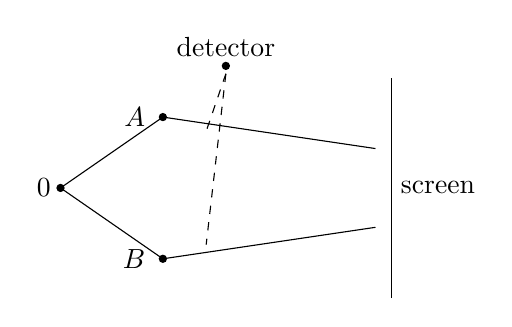
\begin{tikzpicture}[scale=1.0]
\fill (-2,0) circle (1.5pt);
\node[left] at (-2,0) {$0$};
\fill (-0.7,0.9) circle (1.5pt);
\node[left] at (-0.8,0.9) {$A$};
\fill (-0.7,-0.9) circle (1.5pt);
\node[left] at (-0.8,-0.9) {$B$};
\draw (-2,0) -- (-0.7,0.9);
\draw (-2,0) -- (-0.7,-0.9);
\draw (-0.7,0.9) -- (2.0,0.5);
\draw (-0.7,-0.9) -- (2.0,-0.5);
\draw (2.2,-1.4) -- (2.2,1.4);
\node[right] at (2.2,0) {screen};
\fill (0.1,1.55) circle (1.5pt);
\node[above] at (0.1,1.55) {detector};
\draw[dashed] (0.1,1.45) -- (-0.15,0.72);
\draw[dashed] (0.1,1.45) -- (-0.15,-0.72);
\end{tikzpicture}
\caption{对称探测器放置的干净重构：两条路径产生相同的探测器态。}
\end{figure}

\begin{classroomqa}
\lecturetimestamp{00:27:55}
\audiencequestion{在干涉消失之前，必须有人实际读取辅助自旋吗？}
\lecturerresponse{不。电子已经将其路径与自旋关联起来。人们可以重置探测器，一次一个电子地重复实验，并且只检查屏幕击中点的分布。即使没有人读取自旋，条纹也不存在；重要的是物理记录，而不是人类对它的意识。}
\end{classroomqa}

\begin{classroomqa}
\lecturetimestamp{00:29:36}
\audiencequestion{足够轻的反弹板会破坏干涉吗？}
\lecturerresponse{会，如果反弹将板移到两条路径的正交动量态。如果移动后的波包仍然重叠，破坏就只是部分的。质量本身不是判据；最终板态的可区分性才是。}
\end{classroomqa}

辐射提供了另一种不完美的记录器。被加速的带电粒子可能发射光子。在\(A\)附近发射的辐射不必与在\(B\)附近发射的辐射处于相同状态，因此电磁场可以保留路径信息。对于缓慢偏转的电子，发射概率可能很小；讲座使用大约百分之一事件的示意性估计。更强的加速度使辐射以及因此导致的对比度损失更可能发生。要点是定性的：即使未被观测的光子也能带走相干性。

\begin{classroomqa}
\lecturetimestamp{00:32:00}
\audiencequestion{在对比度不完美的真实实验中，如何推断干涉概率？}
\lecturerresponse{人们多次重复实验，并根据相对频率估计屏幕分布。有限样本和环境记录会在名义上的暗区留下残余计数。推断的概率分布随着试验次数增加而改善，而退相干过程会降低物理条纹对比度。}
\end{classroomqa}

\begin{classroomqa}
\lecturetimestamp{00:33:13}
\audiencequestion{任何确定路径的可能性都会破坏全部干涉吗？}
\lecturerresponse{完全的可区分性会将其彻底破坏。部分信息则导致部分损失。一个只略微旋转的探测器留下两个非正交的记录态，因此当读取探测器时，一条路径变得比另一条更可能，但并非确定；相应地，条纹是被模糊而非被抹去。}
\end{classroomqa}

设\(|E_A\rangle\)和\(|E_B\rangle\)表示任意记录态。屏幕处的组合态可写为
\begin{equation}
|\Psi\rangle
=\sum_m\left(
\psi_m|m\rangle|E_A\rangle
+\phi_m|m\rangle|E_B\rangle
\right).
\end{equation}
忽略记录系统则给出
\begin{align}
P(m)
&=|\psi_m|^2+|\phi_m|^2 \\
&\quad
+\psi_m^*\phi_m\langle E_A|E_B\rangle
+\phi_m^*\psi_m\langle E_B|E_A\rangle.
\end{align}
因此重叠\(\langle E_A|E_B\rangle\)就是相干因子。相同的记录保持完全干涉；正交的记录将其消除；中间的重叠给出中间的可见度。

\begin{classroomqa}
\lecturetimestamp{00:34:12}
\audiencequestion{如果光子只是偶尔发射，那么当只保留光子发射事件时会发生什么？}
\lecturerresponse{该选定的子系综通常具有较差的干涉，因为光子携带路径信息。损失不必是完全的：从两个开口发射的光子波包本身可能重叠，因此即便是辐射记录也可能无法完全正交。}
\end{classroomqa}

环境轰击将这一机制放大。空气分子、环境光子和周围物质持续获得宏观位置的记录。一个人或月球不会保持可见地展布为相干的位形叠加：质量减缓自由展布，而持续的环境纠缠抑制宏观分离备选之间的可观测干涉。

\begin{classroomqa}
\lecturetimestamp{00:36:02}
\audiencequestion{这已经是一种测量理论，而不仅仅是又一次使用\emph{波包坍缩}这一说法吗？}
\lecturerresponse{它是在一个刻意精确的示例中的机制。在仅电子的描述中，坍缩意味着丢弃非对角\(\psi^*\phi\)项。在复合描述中无需任何特设的删除：与正交仪器态的纠缠使这些项无法用于仅对电子的测量。更复杂的示例应追溯回这一结构。}
\end{classroomqa}

\begin{classroomqa}
\lecturetimestamp{00:38:04}
\audiencequestion{一个使路径自然弯曲的引力场会改变辐射论证或干涉规则吗？}
\lecturerresponse{详细的辐射可能改变，而量子力学在路径测量之前并不指定单一锐利的轨迹。一般结论不变：只有保留可区分路径信息的自由度才会抑制干涉。在更详细的回答有意义之前，必须指定具体的仪器。}
\end{classroomqa}

\begin{classroomqa}
\lecturetimestamp{00:39:44}
\audiencequestion{这种干涉与经典电磁波的干涉不同吗？}
\lecturerresponse{对于许多光子，观测到的图样与电磁场的普通波干涉一致。单粒子实验显示了更深刻的量子陈述：光子和电子以单个事件到达，而它们的量子振幅发生干涉。对于电子，相关的波是电子波函数，而非电磁波。}
\end{classroomqa}

\begin{classroomqa}
\lecturetimestamp{00:40:45}
\audiencequestion{初始波中瞄准\(A\)与\(B\)之间的部分会怎样？}
\lecturerresponse{在这个刻意离散的模型中，势垒的其余部分被阻挡。那些部分被反射，不对透射的屏幕振幅作出贡献。该模型隔离出两个透射备选，而不声称真实光束只有两个动量分量。}
\end{classroomqa}

\section{猫、屏幕与可移动切割}

同样的数学适用于Schr\"odinger的猫。设枪具有未发射和已发射的状态\(|U\rangle\)和\(|F\rangle\)，并设猫具有活和死的状态\(|L\rangle\)和\(|D\rangle\)。从一只活猫和一支未发射的枪出发，相互作用可能产生
\begin{equation}
|\Psi_{\mathrm{cat}}\rangle
=\alpha|L,U\rangle+\beta|D,F\rangle.
\end{equation}
仅猫本身并不处于相干态\(\alpha|L\rangle+\beta|D\rangle\)。它与一支已记录备选的枪纠缠。观察枪可以揭示猫的分支，而正交的枪记录消除了猫子系统中普通的活--死干涉。

\begin{classroomqa}
\lecturetimestamp{00:41:18}
\audiencequestion{猫本身是否处于既死又活的叠加态？}
\lecturerresponse{并非在简单的孤立意义上如此。猫--枪这一复合系统处于相互关联的备选状态的叠加之中：猫活着时枪未开火，猫死了时枪已开火。猫这一子系统与携带记录的枪纠缠在一起，正如电子的路径与辅助自旋纠缠在一起一样。}
\end{classroomqa}

最终屏幕也必须被当作一台仪器来处理。一个电子到达\(m\)处，可能会使一个照相乳胶颗粒变黑、使闪烁体发出一个光子，或者使一排局域二态器件中的一个探测器发生翻转。该标记便与到达位置关联起来。

\begin{classroomqa}
\lecturetimestamp{00:43:38}
\audiencequestion{为什么我们可以谈论最终屏幕上的概率，而不是永远只携带态矢量？}
\lecturerresponse{概率公设将\(\langle\Pi_m\rangle\)赋予性质\emph{到达\(m\)}。为了完成物理实验，屏幕随后留下一个位置记录。投影算符给出概率；变黑、闪烁或局域探测器的翻转则实现了正在被收集其统计数据的测量。}
\end{classroomqa}

\begin{classroomqa}
\lecturetimestamp{00:45:00}
\audiencequestion{为什么要讨论屏幕测量，却不讨论通过\(A\)或\(B\)的概率？}
\lecturerresponse{只有安装路径记录器，才能赋予并检验路径概率。没有这样的记录，各备选路径保持相干，必须作为振幅相加。在屏幕处，则假定有一台位置灵敏的仪器。区别不在于某个享有特权的时间，而在于是否安排了相应的测量相互作用。}
\end{classroomqa}

系统与仪器之间的边界可以移动。把一位具有记录态\(|O_u\rangle\)和\(|O_d\rangle\)的观察者包括进来；于是
\begin{equation}
|A,u\rangle+|B,d\rangle
\longrightarrow
|A,u,O_u\rangle+|B,d,O_d\rangle.
\end{equation}
另一位观察者又可以依次与第一位关联起来。猫箱中的烟雾、枪、猫、Schr\"odinger以及维格纳，全都可以被纳入一条更长的纠缠链中。无论这条切割线画在哪里，关联都必须保持一致：如果维格纳后来问Schr\"odinger他看到了什么，他们的记录会一致。

\begin{classroomqa}
\lecturetimestamp{00:47:24}
\audiencequestion{系统究竟应当在哪里结束，进行测量的观察者又应当从哪里开始？}
\lecturerresponse{量子力学并不选定一个唯一的方便切割。人们可以对仅含电子的描述作坍缩，也可以把探测器包括进来并对一个更大的描述作坍缩，或者把一位观察者包括进来并再次扩大纠缠态。物理上的要求是所有可及概率与记录的一致性，而不是一个唯一的记账边界。}
\end{classroomqa}

\begin{classroomqa}
\lecturetimestamp{00:49:47}
\audiencequestion{不确定性原理之所以介入，是因为测量路径会扰动事件吗？}
\lecturerresponse{是的。反冲的例子明确地建立了这一联系：板的局域化产生动量不确定性，这可以阻止微小的路径相关反冲变得可区分。更一般地说，量子测量只有在系统--仪器纠缠改变了态之后才算完成，而这种改变可以改变后来的干涉。}
\end{classroomqa}

这标志着与经典理想之间的鲜明对比。在经典情形中，人们设想可以把测量做得任意轻柔，以可忽略的扰动提取信息。而在这里，提取路径信息需要与一台仪器建立关联。这是联合态的真正改变，并且会改变对后来干涉实验的答案。

\begin{classroomqa}
\lecturetimestamp{00:52:06}
\audiencequestion{如果\(A\)与\(B\)之间的间距变得非常大，会发生什么？}
\lecturerresponse{并不存在一条普遍的新规则。在这种源与势垒的几何构型中，到达非常遥远的开口的振幅可能只是变得很小，因此大多数粒子会打在受阻区域上。除了\(\psi_m\)和\(\phi_m\)中这类依赖于仪器的变化之外，仅凭间距本身并不能决定相干性是否存活。}
\end{classroomqa}

\begin{classroomqa}
\lecturetimestamp{00:53:04}
\audiencequestion{量子演化的线性是根本上精确的吗，自然又为什么要使用它？}
\lecturerresponse{线性是量子力学的一个经验基础。微小的非线性修正极难做到逻辑上自洽，而且往往会破坏这一结构。物理命题为何遵循子空间的逻辑而非经典集合的逻辑，其更深层的原因在此并未给出；本讲把它当作自然的一个事实来对待。}
\end{classroomqa}

\begin{classroomqa}
\lecturetimestamp{00:54:53}
\audiencequestion{后来的观测能否揭示先前的路径，从而改变是否发生干涉？}
\lecturerresponse{如果后来的观测能够揭示路径，那么某个物理自由度必定已经保存了依赖于路径的记录。该记录已经影响相干性；并不需要有人去读取它。因果性仍必须得到遵守，而一个抽象的延迟选择主张若不指明完整的时空安排与装置，就无法得到裁定。}
\end{classroomqa}

\begin{classroomqa}
\lecturetimestamp{00:56:47}
\audiencequestion{如果把一个气泡室紧接在开口之后放置，会怎样？}
\lecturerresponse{一条能区分两条出射路径的径迹就是一个明确的标记，因此它会破坏二者的干涉。一层很薄的路径记录层就足够了。如果下游装置没有保留足够的信息来推断先前的开口，那么它并不会自动充当which-path探测器。}
\end{classroomqa}

\begin{classroomqa}
\lecturetimestamp{00:59:29}
\audiencequestion{如果世界已经高度纠缠，干涉实验怎么可能从非纠缠的系统开始？}
\lecturerresponse{制备过程必须对相关自由度进行足够好的隔离、重置或条件化，使得各备选情形从相同的环境记录出发。如果先前的气泡室径迹仍与路径相关联，就不能简单地将其忽略。干涉要求受控系统与相关记录器之间具有类积的初始关系。}
\end{classroomqa}

\begin{classroomqa}
\lecturetimestamp{01:01:04}
\audiencequestion{测量之后，实际的非纠缠从何而来？}
\lecturerresponse{以某个确定的观测结果为条件。如果自旋被发现朝上，观测者就保留分支\(|A,u\rangle\)，并在工作描述中丢弃另一备选。该条件化后的积态可以用作新的起点。包含观测者的完整态可能仍然纠缠，但相对于被记录的结果，所选定的制备是确定的。}
\end{classroomqa}

这种嵌套层级并不解决所有解释性问题，但它使操作上的一致性变得可见。系统、探测器、观测者以及观测者的观测者都可以被纳入。无论描述在何处切开，正确关联的记录之后都不会彼此矛盾。

\section{从纠缠到熵}

讨论在测量问题上走得比计划更远，但它暴露出了下一个问题：纠缠的程度如何测量？处于积态
\begin{equation}
|u\rangle\otimes|u\rangle
\end{equation}
的两个自旋并不纠缠。每个子系统都有自己的确定态，观测其中一个不会提供关于另一个的新信息。纠缠态不会以这种方式分解。标准的定量诊断将是纠缠熵，但我们首先需要通常的熵概念，然后才是它的量子形式。

\section{经典熵作为缺失的信息}

从一个具有\(N\)个可能状态的有限集的经典系统开始。这里的熵是系统连同我们对它的知识的一种性质。假设我们所知道的只是系统占据\(n\)个等概率状态之一。那么
\begin{equation}
S=\log n.
\end{equation}
如果\(n=1\)，状态是已知的，且\(S=0\)。如果\(n=N\)，除了状态空间本身之外一无所知，熵为最大，\(S_{\max}=\log N\)。

对数以相加的方式计算独立的是--否选择。对于\(M\)个经典自旋，有\(2^M\)种构型，因此
\begin{equation}
\log(2^M)=M\log 2.
\end{equation}
因此，在选取对数底的意义上，熵计算的是描述中缺失的二元信息量。

对于一般的概率分布\(p_i\)，合适的定义是
\begin{equation}
S=-\sum_i p_i\log p_i.
\end{equation}

\begin{classroomqa}
\lecturetimestamp{01:14:17}
\audiencequestion{为什么熵公式中有一个负号？}
\lecturerresponse{每个非零概率都满足\(0<p_i\leq 1\)，所以\(\log p_i\leq 0\)。负号使熵非负。在\(p_i=0\)处，贡献由极限\(p_i\log p_i\to0\)定义。}
\end{classroomqa}

对于等概率分布
\begin{equation}
p_i=
\begin{cases}
1/n, & i\in\mathcal N,\\
0, & i\notin\mathcal N,
\end{cases}
\qquad |\mathcal N|=n,
\end{equation}
一般公式变为
\begin{align}
S
&=-n\left(\frac1n\right)\log\left(\frac1n\right)\\
&=\log n.
\end{align}
因此它重现了初等的计数定义。一个以确定性集中于某一状态的分布有\(S=0\)。

\begin{figure}[htbp]
\centering
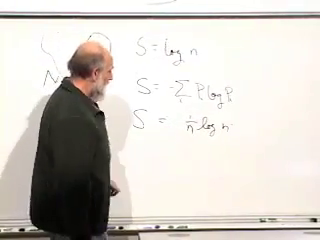
\includegraphics[width=0.66\textwidth]{lecture_07_figure_07.png}
\caption{黑板上汇集了\(S=\log n\)、香农公式以及等概率检验。}
\lectureframe{01:16:08}
\end{figure}

\begin{classroomqa}
\lecturetimestamp{01:17:35}
\audiencequestion{一个具有\(N\)个状态的系统所能具有的最大熵是多少，而在那种情况下已知的是什么？}
\lecturerresponse{最大值是\(\log N\)，由均匀分布\(p_i=1/N\)达到。人们仍然知道系统是什么，因此知道它的状态空间；未知的是它占据这\(N\)个状态中的哪一个。}
\end{classroomqa}

差值
\begin{equation}
I=S_{\max}-S
\end{equation}
就是这种计数意义下的可用信息。熵与信息是同一本账的两面：熵记录的是本可区分状态、但我们却无法获得的信息。

\section{迹：求和的量子替代}

对于算符\(M\)以及任意完备正交归一基\(\{|i\rangle\}\)，定义
\begin{equation}
\operatorname{Tr}M
=\sum_i\langle i|M|i\rangle.
\end{equation}

\begin{figure}[htbp]
\centering
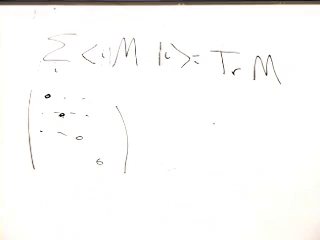
\includegraphics[width=0.68\textwidth]{lecture_07_figure_08.png}
\caption{迹写成对角矩阵元之和。}
\lectureframe{01:21:20}
\end{figure}

尽管这个定义是用一组基写出的，但结果与基无关。对于厄米算符，可以选取本征基，此时
\begin{equation}
\operatorname{Tr}M=\sum_i\lambda_i.
\end{equation}
本征值、从而它们的和，并不依赖于用来表示该算符的坐标。

\begin{classroomqa}
\lecturetimestamp{01:23:04}
\audiencequestion{把一个矩阵化为对角形式是否意味着它有逆？}
\lecturerresponse{不。对角形式展示的是本征值；可逆性是一个独立的条件。一个对角矩阵可逆，当且仅当它的对角本征值中没有零。厄米矩阵即使有些本征值为零，也仍然可以对角化。}
\end{classroomqa}

休息之后，简要回到经典概率。经典可观测量是位形的函数\(f_i\)，其平均值为
\begin{equation}
\langle f\rangle_{\mathrm{cl}}=\sum_i p_i f_i.
\end{equation}
在量子公式中，迹将取代对各种可能性的求和，算符将取代经典函数，密度矩阵将取代概率分布。

\section{统计混合与密度矩阵}

假设有人把系统制备在某个正交归一基的一个状态上，却不告诉我们选的是哪个状态。他们只给出制备概率---例如，一个自旋以概率\(3/4\)被制备为上，以概率\(1/4\)被制备为下。这不是相干叠加
\begin{equation}
\sqrt{\frac34}|u\rangle+\sqrt{\frac14}|d\rangle,
\end{equation}
因为没有制备任何相对相位。它是确定状态的统计混合。即使已知一个纯态，量子概率依然存在；这里还额外存在关于制备了哪个纯态的不确定性。

\begin{figure}[htbp]
\centering
\includegraphics[width=0.66\textwidth]{lecture_07_figure_06.png}
\caption{从指定 ket 到系综描述的概念转变。}
\lectureframe{01:29:43}
\end{figure}

如果状态\(|i\rangle\)以概率\(\rho_i\)被制备，则密度算符为
\begin{equation}
\rho=\sum_i\rho_i|i\rangle\langle i|.
\end{equation}
在制备基中，
\begin{equation}
\rho=
\begin{pmatrix}
\rho_1&0&0&\cdots\\
0&\rho_2&0&\cdots\\
0&0&\rho_3&\cdots\\
\vdots&\vdots&\vdots&\ddots
\end{pmatrix}.
\end{equation}

\begin{figure}[htbp]
\centering
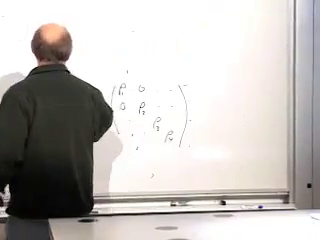
\includegraphics[width=0.68\textwidth]{lecture_07_figure_09.png}
\caption{对角密度矩阵及其归一化条件。}
\lectureframe{01:32:12}
\end{figure}

它的本征值是实的且非负的，而概率的归一化变为
\begin{equation}
\operatorname{Tr}\rho=\sum_i\rho_i=1.
\end{equation}

设\(F\)为厄米可观测量。系综期望值为
\begin{equation}
\langle F\rangle=\operatorname{Tr}(F\rho).
\end{equation}

\begin{figure}[htbp]
\centering
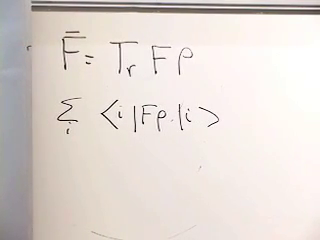
\includegraphics[width=0.68\textwidth]{lecture_07_figure_10.png}
\caption{迹期望值\(\langle F\rangle=\operatorname{Tr}(F\rho)\)。}
\lectureframe{01:35:05}
\end{figure}

为了恢复通常的加权平均，在\(\rho\)对角化的基中计算迹，并插入单位分解：
\begin{align}
\operatorname{Tr}(F\rho)
&=\sum_i\langle i|F\rho|i\rangle\\
&=\sum_{i,j}\langle i|F|j\rangle
               \langle j|\rho|i\rangle\\
&=\sum_i\rho_i\langle i|F|i\rangle.
\end{align}
因此，每个纯态期望值都由相应状态被制备的概率加权。

迹具有循环性质
\begin{equation}
\operatorname{Tr}(AB)=\operatorname{Tr}(BA),
\end{equation}
即使\(A\)与\(B\)不对易。因此\(\operatorname{Tr}(F\rho)=\operatorname{Tr}(\rho F)\)。

\section{量子熵与延后的回报}

密度矩阵的熵为
\begin{equation}
S(\rho)=-\operatorname{Tr}(\rho\log\rho).
\end{equation}
对于厄米正算符，诸如\(\log\rho\)这样的函数通过其本征值来定义。如果
\begin{equation}
\rho=\sum_i\rho_i|i\rangle\langle i|,
\end{equation}
那么
\begin{equation}
\log\rho=\sum_{\rho_i>0}(\log\rho_i)|i\rangle\langle i|,
\end{equation}
因此
\begin{equation}
S(\rho)=-\sum_i\rho_i\log\rho_i.
\end{equation}

\begin{figure}[htbp]
\centering
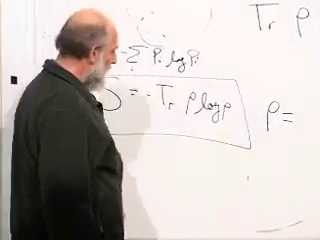
\includegraphics[width=0.68\textwidth]{lecture_07_figure_11.png}
\caption{经典熵公式改写为\(S=-\operatorname{Tr}(\rho\log\rho)\)。}
\lectureframe{01:41:25}
\end{figure}

一个已知纯态具有密度算符
\begin{equation}
\rho_\psi=|\psi\rangle\langle\psi|,
\end{equation}
其本征值为\(1,0,\ldots\)，所以\(S(\rho_\psi)=0\)。这并不意味着对\(|\psi\rangle\)的每一次测量都有确定的结果。它意味着关于所制备的状态不存在额外的统计无知。在相反的极端，
\begin{equation}
\rho=\frac{I}{d}
\qquad\Longrightarrow\qquad
S(\rho)=\log d,
\end{equation}
其中\(d=\dim\mathcal H\)。最大混合态给每个正交方向赋予相同的权重。

与纠缠的联系如今已很接近，但尚未完全解决。假设一个复合系统 \(AB\) 处于联合态，并且所有实验都局限于 \(A\)。必定存在一个对象，它能在忽略 \(B\) 的同时，重现可在 \(A\) 上获得的一切期望值。该对象就是 \(A\) 的密度矩阵。如果联合态可因式分解，则 \(A\) 的密度矩阵是纯态且熵为零。如果 \(A\) 与 \(B\) 纠缠，则 \(A\) 的密度矩阵一般是混合态且熵非零。构造该约化密度矩阵并计算其熵，是留待下一讲的任务。
